\documentclass[12pt]{report}

\usepackage[T1]{fontenc}
\usepackage[utf8]{inputenc}
\usepackage{graphicx}
\usepackage{amssymb, amsmath, amsbsy}

\begin{document}

\begin{center}
{\Huge \textbf{Calcular los parametros de circuitos de activacion de trasistores de potencia  .}\\}
\Large{Enesto Alonso Partida López\\ Universidad Politecnica De La Zona Metropolitana De Guadalajara\\ Mecatronica 4 A\\ Septiembre-diciembre 2019}\\
{29 de octubre 2019 }\\
\end{center}
\begin{center}



\includegraphics[scale=1]{../../../../Downloads/upzmg.jpg} 
\end{center}
\newpage
{\huge \textbf{¿Que es un Transistor?}\\}


{\Large El transistor es un dispositivo electrónico semiconductor utilizado para entregar una señal de salida en respuesta a una señal de entrada. Cumple funciones de amplificador, oscilador, conmutador o rectificador. }\\



{\huge \textbf{¿Tipos de Trasistores?  }}\\

{\Large Los transistores están formados por la unión de tres cristales semiconductores, dos del tipo P uno del tipo N (transistores PNP), o bien dos del tipo N y uno del P (transistores NPN). }\\
\begin{center}
\begin{figure}[hbtp]
\caption{Transisitor NPN y PNP}
\centering
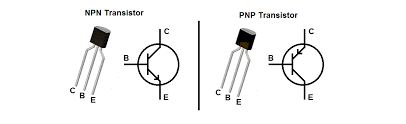
\includegraphics[scale=1]{../../../../Downloads/descragas/transistor.png}
\end{figure}

\end{center}


{\huge \textbf{¿Cómo calcuar la resistencia para un transistor?}\\
{\Large Un transistor puede ser activado (saturación) o desactivado (corte) desde un microcontrolador, pero es necesario poner una resistencia entre la pata del micro y la base del transistor.
Lo primero que se tiene que tener en cuenta es el tipo de carga con la que se trabajara, para posteriormente elegir entre un PNP o bien un NPN. Ya que no es lo mismo usar un BC107 que permite tensiones de hasta 45 V. y corrientes de hasta 100 mA. que un 2N3055 que permite tensiones de hasta 60 V. y corrientes de hasta 15 A.}
\begin{center}
\begin{figure}[hbtp]
\centering
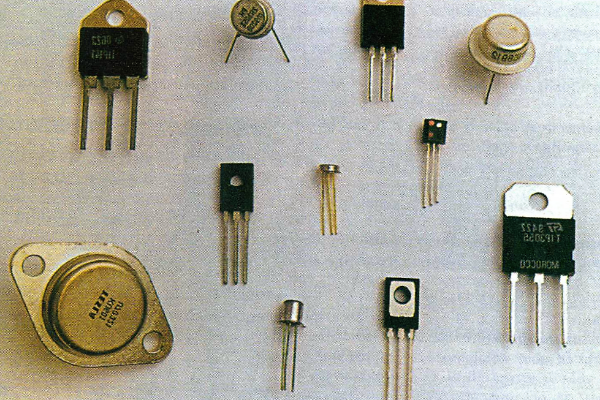
\includegraphics[scale=.7]{../../../../Downloads/descragas/transisitores.png}
\caption{Tipos de Transistores}
\end{figure}

\end{center}

{\Large Cuando se tiene el transistor lo que sigue es encontrar la resistencia correcta para dicho componente la cual se puede obtener mediante una formula:\\
}

\begin{equation}
R=\dfrac{Voltaje - 0.7}{\dfrac{corriente}{hFe}}
\end{equation}
{\Large Donde:\begin{itemize}
\item Voltaje: Es la tensión que proporciona el microcontrolador. Se resta 0,7 V. porque es la caída de tensión típica entre la base y el emisor de un transistor, aunque lo puedes mirar en el datasheet del transistor como Vbe.
\item Coriente: la corriente que consume el circuito
\item hFe: Es la ganancia de corriente (current gain.
\end{itemize}}
\newpage
{\huge \textbf{Bibliografia:}\\}\\
{\large
@online{SISTEMAS O.R.P,
author = {Diseño digital},
title = {Calcular la resistencia para un transistor accionado por un microcontrolador},
year = {2011},
url = {https://www.sistemasorp.es/2011/10/05/calcular-la-resistencia-para-un-transistor-accionado-por-un-microcontrolador/},
OPTsubtitle = {Calcular la resistencia para un transistor accionado por un microcontrolador
OPTversion = {copyright},
OPTdate = {5},
OPTmonth = {octubre},

}
}

\end{document}